\section{App utenti}
\subsection{Introduzione}
Questa parte del documento è orientata agli utenti che utilizzano l'applicazione Android.

\subsubsection{Scopo del prodotto}
L'applicazione Android è sviluppata per due diverse tipologie di utente ovvero il dipendente e l'addetto alle pulizie.

In generale offre all'utente le seguenti funzionalità:
\begin{itemize}
	\item \textbf{Login:} L'utente ha la possibilità di autenticarsi inserendo il proprio username e password; \\
	\item \textbf{Logout:} L'utente ha la possibilità di deautenticarsi premendo sull'elemento della lista "Logout" del menù principale in alto a destra. \\
\end{itemize}

Per quanto riguarda il dipendente, l'applicazione offre i seguenti servizi:
\begin{itemize}
	\item \textbf{Scansione:} Il dipendente ha la possibilità di scansionare una postazione per poter visualizzare lo stato di essa e altre informazioni come le prenotazioni associate ad essa; \\
	\item \textbf{Occupazione:} Il dipendente dopo aver scansionato una postazione può occuparla se questa è prenotata da lui o è libera e igienizzata; \\
	\item \textbf{Igienizzare:} Il dipendente dopo aver scansionato una postazione la può igienizzare se questa risulta non igienizzata; \\
	\item \textbf{Lista prenotazioni:} Il dipendente può visualizzare le prenotazioni effettuate premendo sull'elemento della lista "Visualizza prenotazioni" del menù principale in alto a destra; \\
	\item \textbf{Disdire prenotazione:} Il dipendente può disdire una prenotazione dopo che è entrato nella pagina in cui visualizza tutte le prenotazioni effettuate; \\
	\item \textbf{Guida:} Il dipendente può visualizzare la guida premendo sull'elemento della lista "Guida" del menù principale in alto a destra; \\
	\item \textbf{Prenota postazione:} Il dipendente può prenotare una postazione premendo sull'elemento della lista "Prenota postazione" del menù principale in alto a destra.
	Dopo aver premuto dovrà inserire la data, l'ora di inizio, l'ora di fine e la stanza obbligatoriamente e in modo facoltativo anche il nome del collega.
	Una volta premuto sul bottone "Cerca", se è stato inserito il nome del collega, visualizzerà tutte le sue prenotazioni effettuate nella stanza, nel range orario e nella data inseriti e scorrendo sotto visualizzerà tutte le postazioni di quella stanza con il loro stato e potrà decidere quale prenotare se disponibile. \\	
\end{itemize}

Per l'addetto alle pulizie l'applicazione offre le seguenti funzionalità:
\begin{itemize}
\item \textbf{Visualizzare stanze da igienizzare:} \\
\item \textbf{Visualizzare postazioni da igienizzare:} \\
\item \textbf{Marcare stanze come igienizzate:} \\
\item \textbf{Marcare postazioni come igienizzate:} \\
\end{itemize}



\subsection{Requisiti e installazione}

\subsubsection{Requisiti}
Per poter sviluppare sul proprio PC l'applicazione sono necessari i software e gli strumenti indicati in questa pagina. I software da installare saranno divisi in base al loro scopo.

Per scaricare il codice sorgente dell'applicazione bisogna andare nella pagina di GitHub che lo ospita, che si trova \href{https://github.com/DPCMGroup/bc19-mobile}{qui}, cliccare su Clone or download e successivamente premere su Download ZIP.

Un'alternativa più efficace a questo procedimento è scaricare il progetto tramite Git. Se non si dispone di Git è possibile scaricarlo seguendo quanto indicato nella sezione Source Code Management. Per scaricare il progetto in questo modo, digitare il seguente comando tramite un terminale o prompt dei comandi nel sistema in uso:\\ \\
\textbf{https://github.com/DPCMGroup/bc19-mobile.git}

\subsubsection{Prerequisiti hardware e software}
Le tecnologie utilizzate per sviluppare l'applicazione Android richiedono parecchie risorse nel loro uso contemporaneo. Si consiglia quindi di avere un computer con processore almeno quad-core e una memoria RAM di almeno 8 GB.

\subsubsection{Ambiente di sviluppo}

\paragraph{Android Studio}
L'applicazione è stata sviluppata utilizzando l'ambiente di sviluppo Android Studio, attualmente alla versione 4.1.3.
\\
\\
\textbf{Installazione di Android Studio su Windows}
\\
È possibile scaricare Android Studio su Windows visitando il sito ufficiale riportato \href{https://developer.android.com/studio}{qui}, andando alla sezione "Android Studio downloads".
Per eseguire l'installazione, bisognerà seguire la guida riportata nella sezione Windows cliccando nel seguente link \href{https://developer.android.com/studio/install}{qui}.
\\
\\
\textbf{Installazione di Android Studio su MacOS}
\\
La guida per scaricare Android Studio per MacOS è identica a quella per Windows.
Per eseguire l'installazione, invece, bisognerà seguire la guida riportata nella sezione Mac cliccando nel seguente link \href{https://developer.android.com/studio/install}{qui}.
\\
\\
\textbf{Installazione di Android Studio su Ubuntu (e derivate, e altri derivati di Debian)}
\\
La guida per scaricare Android Studio per Linux è identica a quella per Windows e MacOS.
Per eseguire l'installazione, invece, bisognerà seguire la guida riportata nella sezione Linux cliccando nel seguente link \href{https://developer.android.com/studio/install}{qui}.
\\
\subsubsection{Linguaggi utilizzati}

\paragraph{Kotlin}
\textbf{Installazione di Kotlin su Windows}
\\
È possibile installare Kotlin su Windows visitando \href{https://plugins.jetbrains.com/plugin/6954-kotlin/versions}{questa pagina}.
Il link porta alla pagina di jetBrains e ti permette di installare l'ultima versione di Kotlin disponibile anche con il plugin su Android Studio.
\\
\\
\textbf{Installazione di Kotlin su MacOS}
\\
L'installazione per MacOS è identica a quella per Windows.
\\
\\
\textbf{Installazione di Kotlin su Ubuntu (e derivate, e altri derivati di Debian)}
\\
È possibile installare Kotlin su sistemi Linux in modo identico a MacOs e Windows.

\paragraph{XML}
La configurazione dell'applicazione e alcune sue dipendenze sono gestite tramite un file denominato AndroidManifest.xml. Inoltre, lo sviluppo di applicazioni Android richiede una cartella di progetto denominata "res" che contiene tutti i file XML per gestire risorse come layout, immagini, menu, stringhe e altro. Quindi è richiesta una buona conoscenza del linguaggio XML.

\subsubsection{Librerie utilizzate}

\paragraph{Kotlin MVP auto}
Viene utilizzata il plugin Kotlin MVP auto per generare in automatico una porzione di codice che rispetti l'architettura MVP. Il plugin è scaricabile a \href{https://plugins.jetbrains.com/plugin/12265-kotlin-mvp-auto}{questa pagina}.
Per poterla usare vengono usate le seguenti dipendenze da aggiungere a build.gradle(:app):\\
\begin{itemize}
	\item implementation 'com.github.cn-ljb:kotlin-mvp-lib:1.2.0'; \\
	\item implementation 'com.github.cn-ljb:netlib:1.0.1'; \\
	\item implementation 'com.github.cn-ljb:daolib:1.0.1'. \\
\end{itemize}

\paragraph{OkHttp}
OkHttp è una libreria che permette di effettuare richieste al server.
Per usarla è necessario aggiungere nel file build.gradle(:app) la dipendenza:\\
implementation 'com.squareup.okhttp3:okhttp:3.8.1'


\subsubsection{Source code management}
Per poter effettuare il versionamento del codice sorgente è richiesto di utilizzare Git. Per poterlo installare è necessario recarsi a \href{https://git-scm.com/downloads}{questa pagina}.
Non è strettamente necessario, ma è consigliato per integrare le proprie modifiche nel repository.

\subsubsection{Build automation}
La build automation (ovvero la gestione del processo di build) è affidata a Gradle, integrato e utilizzato in Android Studio. I file di build sono due: uno per tutto il progetto ed uno per il solo modulo app.
Tramite Gradle il progetto dell'applicazione viene compilato, testato ed eseguito attraverso l'IDE Android Studio.


\subsection{Estendibilità}

\subsubsection{Creazione di un metodo}
Tramite l'utilizzo dell'architettura Model View Presenter è facile da implementare dei nuovi metodi separandoli con la business logic e la vista e in seguito creare i rispettivi collegamenti utilizzando il presenter.


\subsection{Architettura}
Il modello architetturale scelto è il Model View Presenter che è fortemente consigliato per chi sviluppa delle applicazioni per dispositivi Android. Il MVP fornisce un modo semplice per mostrare la struttura del prodotto garantendo modularità, testabilità e in generale una base di codice più pulita e gestibile. Ne deriva quindi l'applicazione del paradigma separation of concerns, che separa la responsabilità tra le differenti parti del pattern.
Come detto in precedenza verrà usato il plugin \href{https://git-scm.com/downloads}{Kotlin MVP auto} per generare in automatico codice che rispetti l'architettura.
\begin{figure}[H]
	\centering
	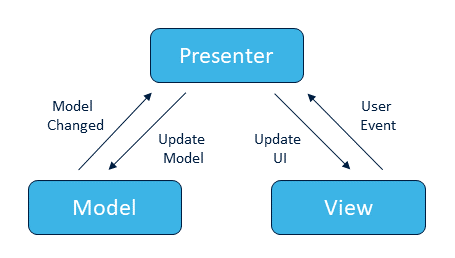
\includegraphics[width=16cm]{res/images/mvp.png}
	\caption{Model-View-Presenter}
	\label{fig:Model-View-Presenter}
\end{figure}

\subsubsection{Model}
Il Model è la parte dell'archittetura che ha il compito di gestire i dati e rappresenta il layer di persistenza dell'applicazione. La maggior parte delle operazioni e dei controlli vengono svolti al suo interno. Contiene anche i metodi che avviano le connessioni alle API ed interagiscono con esse eseguendo numerose funzionalità. Vi sono, ad esempio, i metodi che consentono la comunicazione con il backend.


\subsubsection{View}
La View ha la responsabilità di passare i dati al Presenter. Essa è implementata da:
\begin{itemize}
	\item Attività (Activity); \\
	\item Qualsiasi forma grafica con cui l'utente finale dell'applicazione andrà ad interagire \\	
\end{itemize}

\subsubsection{Presenter}
Il Presenter funge da livello intermedio tra la View e il Model. Tutta la logica di presentazione appartiene ad esso ed è responsabile dell'interrogazione del modello e l'aggiornamento della vista, reagendo alle interazioni che compie l'utente nella UI. Un valore aggiunto è che il Presenter dipende dall'astrazione della View e non dalla sua concretizzazione, quindi non conosce la sua implementazione. Tutto ciò favorisce ad una più facile attività di test.

\subsubsection{Contract}
Il Contract può essere visto come un contratto nel quale vengono definiti tutti i metodi che verranno utilizzati dalla View, dal Presenter e dal Model. Quando si ha intenzione di scrivere una nuova funzionalità, è buona norma scrivere un Contract. Esso descrive la comunicazione tra View-Presenter e Model-Presenter, consentendo una progettazione più pulita e diminuire le dipendenze tra le componenti.
Il Contract è un'interfaccia e contiene le altre interfacce della View, Presenter e Model per garantire le varie comunicazioni.

\subsection{Diagramma dei package}

\subsection{Diagramma delle classi}

\subsection{Diagramma di sequenza}
